\documentclass[11pt]{article}
\usepackage[linktocpage=true]{hyperref}
\usepackage[utf8]{inputenc}
\usepackage[T1]{fontenc}
\usepackage{fixltx2e}
\usepackage{algorithm}
\usepackage{algpseudocode}
\usepackage{listings}
\usepackage[dvipsnames]{xcolor}
\usepackage{hyperref}
\usepackage{graphicx}
\usepackage{wrapfig}

\setlength{\parskip}{3pt}

\widowpenalties 1 10000

\hypersetup{
	linkcolor  = blue!60!black!90!gray,
	citecolor  = blue!60!black!90!gray,
	urlcolor   = blue!60!black!90!gray,
	colorlinks = true
}

\lstset{
  basicstyle=\ttfamily,
  columns=fullflexible,
  breaklines=true,
  tabsize=4
}

\title{%
  \textbf{Althea} \\
	\vspace{3pt}
  \large An incentivized mesh network protocol}
\author{Jehan Tremback, Justin Kilpatrick\\
\texttt{\{jehan,justin\}@altheamesh.com}\\}
\date{May 2017\\
\texttt{v0.4}}
\begin{document}

\maketitle

\begin{abstract}

As the number of connected individuals and devices expands, the ``last mile'' continues to be the greatest challenge both in the connected and developing worlds, representing a disproportionate portion of the cost and difficulty of connecting the world.
 
Althea is meant to operate on the last mile, from a source of internet connectivity (such as an internet exchange point) to the end user, and creates a distributed ISP. The last mile is currently an inefficient market- many areas only have one ISP \cite{fcc}. Althea aims to replace centralized ISPs with a free market of individuals providing connectivity services as part of one decentralized network.
 
We hope that by lowering the barrier of entry to earn money by providing connectivity services we can decrease the cost of of internet access. This could help connect the developing world as well as creating an environment that fosters competition in otherwise monopolistic last mile infrastructure in developed countries.
 
Althea’s goal is for any person to be able to install a piece of equipment, route traffic for others, and receive payment for the service.

\begin{itemize}
\item[--] Switching costs within the system are reduced, as nodes switch between connectivity providers automatically according to a routing protocol which finds a route with the best combination of reliability, bandwidth, and low cost.
 
\item[--] Advertising and marketing costs for the connectivity providers are eliminated, as the only advertisements in this system are the automatic advertisements of price and route quality between nodes. This makes things easy for new entrants.
 
\item[--] Contract and billing costs are eliminated by payment channels. Payment channels allow one to make micropayments with very low overhead.
\end{itemize}

\end{abstract}

\tableofcontents

\section{Overview}
\label{sec:overview}
Althea allows routers to pay each other for bandwidth using cryptocurrency payment channels. An important architectural detail is that nodes only pay neighbors for forwarding packets. On top of this pay-for-forward network, we build a system allowing consumers to pay for internet access. Althea is intended to be used in local ``mesh'' \cite{wcn} networks.

\subsection{Network}

There are a few different types of nodes that participate in Althea:

\begin{itemize}
\item[--] \textbf{Home nodes} are installed by people who want to buy internet access on Althea. You can think of a home node as being similar to the router and/or modem that is installed by a traditional ISP. The difference is that it is independent of any one ISP.
 
Home nodes may be paid by other nodes to forward packets, but without specialized hardware and positioning the income is expected to be be relatively small.

\item[--] \textbf{Intermediary nodes} are installed by people who want to earn money by forwarding internet traffic (connectivity providers). These will typically be more powerful nodes and may be placed in advantageous locations with good line of sight to other nodes. 

\item[--] \textbf{Gateway nodes} are like intermediary nodes, but they are connected to a source of cheap internet bandwidth such as an internet exchange, an internet backbone connection, or even a business-grade connection from a conventional ISP. They act as connection from Althea’s physical layer to the outside internet. However, they are shielded from having to take legal responsibility for traffic on the network by the exit servers.

\item[--] \textbf{Exit servers} are not necessarily part of the local physical network, but can be hosted in a datacenter reachable over the internet. They are connected to gateway nodes over VPN tunnels. Exit servers provide an endpoint to verify quality metrics propagated by nodes in the network. This enables automatic selection of gateway nodes by the routing protocol. Exit servers also take on the legal role of an ISP, performing network address translation to route requests onto the public internet and dealing with copyright complaints etc. This allows gateway nodes to act as pure providers of bandwidth, without having to take on any legal risk resulting from the use of their service.

\end{itemize}

Read more about the network architecture in \autoref{sec:network}.

\subsection{Routing}
In \autoref{sec:routing}, we define a couple of extensions to the Babel routing protocol. Babel was selected because it has several useful properties for our purpose. However, any distance vector routing protocol could be modified to exhibit the properties we require. Distance vector protocols are already used extensively on the internet. One well-known distance vector protocol is BGP \cite{bgp}.
 
Routing in distance vector protocols is based on an advertised connection quality metric. Nodes send an announcement packet stating their identity and existence to the network once every predetermined period. These announcement packets are then passed from node to node. Each node updates the metric to reflect the connection quality between it and the neighbor it got the announcement from. Using this information, each node is able to build up a routing table of the best neighbors to forward packets to to get to any destination on the network.
 
We propose two main additions to distance vector routing:

\begin{itemize}
\item[--] A verifiable quality metric.
\item[--] A price metric.
\end{itemize}

A verifiable quality metric is a connection quality metric that can be verified by a node and the destination that it is sending packets to. Our first extension to Babel allows nodes to verify the metrics advertised by their neighbors.
 
To advertise prices a second metric is added to the routing advertisements, this time containing a ‘price’ value for some arbitrary but agreed upon amount of data transfer. When passing advertisements each node updates the price field with their bid for passing data. Routes are then selected by optimizing the quality metric vs the price metric and paying the selected the full sum required to route all the way to the destination. 

\subsection{Payments}
Each node on the network establishes payment channels with each of its neighbors. A payment channel is a method for two parties to exchange payments trustlessly by signing transactions that alter the balance of an escrow account held by a bank or blockchain (we may use the Ethereum blockchain for Althea) \cite{btcwiki}, \cite{bitcoinj}, \cite{machinomy}. More detail about the functioning of our payment channels can be found in \autoref{sec:payments}.
 
The important thing about a payment channel is that after the channel has been opened, and funds have been placed in escrow, individual payments can be made directly between the two parties without submitting anything to the bank or blockchain. This means that the entire payment can be completed in one packet. Most payment systems need to send another transmission to a bank or blockchain, and wait for it to be confirmed. 
 
Using payment channels, nodes can pay each other in very small increments (on the order of cents or less). This allows them to pay their neighbors to forward data without having to place a lot of trust in their neighbors. Home nodes also open a payment channel with an exit server of their choice. This channel is used to pay the exit server for routing data onto the internet, as well as paying for return traffic back to the node. Read more about exit servers in \autoref{sec:network}.

\subsection{Metering}
Nodes keep track of data they have forwarded for their neighbors, and how much they have been paid. If these two amounts do not match up, they must having some way of cutting off access to the delinquent neighbor. Blocking the neighbor’s MAC address could be one way to accomplish this, but MAC addresses are easily changed and spoofed. Similarly, exit servers must be able to control traffic from home nodes.
 
In \autoref{sec:metering}, we cover the use of tunnels to allow neighbors to verify traffic between one another, as well as allowing exit servers to authenticate traffic from home nodes.

\section{Routing}
\label{sec:routing}
Routing in Althea is based on the Babel routing protocol \cite{babel}. Babel is a distance vector protocol which has proven to be robust and performant. All distance vector protocols are based on a distributed form of the Bellman-Ford pathfinding algorithm \cite{bellmanford}. Nodes first perform some kind of link quality test on the connections to their neighbors. This is known as the ``link cost''. They then share information about which destinations they can reach at which quality (this starts out being only their immediate neighbors).
 
Whenever a node receives information about a destination, it combines this information with the link cost of the neighbor it received this information from. This composite score is known as the ``route metric'', and represents the quality with which the destination can be reached across several hops. The neighbor offering the best metric for a given destination is selected as the next hop. All packets being sent to the destination will go through this neighbor. Babel implements this selection by adding and remove routes from the Linux kernel routing table.
 
From the Babel specification:
\begin{quote}
As many routing algorithms, Babel computes costs of links between any two neighbouring nodes, abstract values attached to the edges between two nodes.  [..]\\
Given a route between any two nodes, the metric of the route is the sum of the costs of all the edges along the route. The goal of the routing algorithm is to compute, for every source S, the tree of the routes of lowest metric to S.
\end{quote}

NOTE: We will use the word ``destination'' to refer to the destination of data packets. Babel refers to this as ``source'', because it is the source of routing packets.

\subsection{Route metric verification}
All current distance vector protocols, including Babel, have a major weakness. All information about link cost and route metrics is provided on a completely trusted and unverified basis. There is nothing stopping any node from claiming that it has the best route to any destination. This is usually not a problem, since most networks today are owned by one entity. In Althea, nodes are owned by many people and entities, all competing to provide the best service. Leaving this vulnerability unaddressed would allow financially-motivated attacks, such as nodes claiming to have better routes than they actually do in an effort to get more business.
 
Babel uses a sequence of ``Hello'' and ``I heard you'' (or ``IHU'') messages to estimate link quality between neighbors. Each node periodically broadcasts a Hello message to all of its neighbors. Each Hello has a sequence number. By looking at the sequence number of each Hello received and comparing it to the last one, neighbors can determine whether they have missed Hello messages from the node. Nodes keep an array of 16 bits for each neighbor corresponding to the last 16 Hello messages, with a 1 representing a received Hello and a 0 representing a missed Hello. From this array, a number called the ``rxcost'' (short for receive cost) is calculated.

This rxcost is then sent back to the neighbor in an IHU message. The neighbor then considers this number the ``txcost'' (short for transmit cost). From these two numbers the overall link cost is calculated using the ETX metric \cite{etx}. From the Babel specification:

\begin{quote}
A node uses a neighbour's Hello history to compute an estimate,
written beta, of the probability that a Hello TLV is successfully
received.  The rxcost is defined as 256/beta.\\

Let alpha be MIN(1, 256/txcost), an estimate of the probability of
successfully sending a Hello TLV.  The cost is then computed by\\

   cost = 256/(alpha * beta)\\

or, equivalently,\\

   cost = (MAX(txcost, 256) * rxcost) / 256.\\

\end{quote}

We propose a modification to the Babel protocol to allow for verification of routes. Our modification involves nodes sending Hellos and IHU messages back and forth to remote destinations. The same cost and metric calculations are performed as with local neighbors. The metric calculated is expected to be close to the overall metric advertised for the destination by the neighbor currently forwarding packets to the destination. This gives us a way to verify the accuracy of advertised routes. If the metric does not match the metric advertised by the selected neighbor, the neighbor’s accuracy score is affected (\autoref{sec:accuracy}), and the metric through this neighbor is adjusted (\autoref{sec:adjustment}).

\subsection{Verification scheduling}
We have the ability to test and verify the routes advertised by neighbors, but we need some way of deciding which routes to verify. Verification runs on a timer. Each verification cycle a node follows this procedure to choose a route $r$ to verify:

\noindent
\begin{minipage}[c]{\textwidth}
\vspace{\abovedisplayskip}
\begin{algorithmic}
\State $D=$ \{ destinations used in the past $x$ seconds \}
\State $d\gets$ \Call{randomSample}{$D$}
\State $R=$ \{ feasible routes to destination $d$ \}
\State $r\gets$ \Call{randomSample}{$R$}
\end{algorithmic}
\vspace{\belowdisplayskip}
\end{minipage}

We start with the set of all destinations that have been used in the past $x$ seconds. $x$ will be set at a reasonable constant, or it could be adjusted to control verification focus. We select a destination $d$ from this set at random. We then get the set of all routes that are feasible and have a destination of $d$. We select a route $r$ from this set at random.

To test the route, we send the destination ``Remote Hello'' packets for some amount of time. The Remote Hello packets are similar to Babel’s local Hello packets, but they also carry information about which neighbor they were sent through. Destinations periodically send ``Remote IHU'' packets to those nodes they have recently received Remote Hello packets from. Similar to Babel’s link cost calculation, the Remote Hello packets are used by the destination to calculate a route cost, and the Remote IHU packets carry this information back. Remote IHU packets also carry back the information about which neighbor the Remote Hello was sent through.

\subsection{Accuracy score}
\label{sec:accuracy}
Once we receive a Remote IHU from a destination, we update the neighbor’s accuracy score $s$ with the following procedure:

\noindent
\begin{minipage}[c]{\textwidth}
\vspace{\abovedisplayskip}
\begin{algorithmic}
\State $d=$ destination that sent the IHU
\State $n=$ neighbor shown by IHU message
\State $c=$ verified route cost shown by IHU message
\State $m=$ advertised route metric of $n$
\State $A=$ \{ accuracy scores of $n$, indexed by destination \}\\
\State $a=$ \Call{min}{$m / c$, 1}
\State $A_d\gets (A_d+a)/2$
\State $s\gets$ \Call{average}{$A$}\\
\If{$s < C_1$}
\State $n$'s routes are removed from routing table
\EndIf
\end{algorithmic}
\vspace{\belowdisplayskip}
\end{minipage}

A per-destination accuracy score $a$ is calculated as the proportion of the verified route cost $c$ to the route metric $m$ advertised by the neighbor $n$. It is then averaged with the current accuracy score for that destination $A_d$. We then take $s$, the average of all active destination accuracy scores for the neighbor. If $s$ drops below some adjustable value $C_1$, the neighbor’s routes are taken off of the kernel routing table.

\subsection{Route metric adjustment}
\label{sec:adjustment}
The above system is used to weed out chronically inaccurate neighbors, but it also supplies us with a stream of correct route metrics. We can use these metrics to improve our routing table even before a given inaccurate neighbor is dropped. When we receive the route cost c above, we can start using it instead of the neighbor’s advertised metric when selecting routes. We continue using c for a duration $D$.
 
How long to make $D$? If $D$ is too short, then nodes will go right back to trusting an inaccurate metric that they recently had to correct. If $D$ is too long, then nodes will miss out on legitimate updates about newly improved routes.
					
To strike the right balance, exponentially increasing time-out will be used for bandwidth corrections beyond a small tolerance. A node that has participated in a correction will record the time $T_{last}$ it last performed a correction for a given route and the size of the correction $\delta$. When participating in another correction on the same route the duration $D$ to apply the bandwidth correction will be determined as:

\[
D = \frac{C_1}{T_{now} - T_{last}}^{\delta C_2}
\]

Where $C_1$ and $C_2$ are constants to be adjusted and hardcoded. This formula will make it take longer to go back to using a neighbor’s advertised metrics if the advertised metrics needed to be corrected recently, and/or required a large correction.

\subsection{Price metric}
We also need a way to propagate a price for each route, and take this price into account when making forwarding decisions. Babel already includes a mechanism for adding arbitrary ``External Sources of Willingness''. This works by having nodes add a number to the metric they have calculated for a route. This doesn’t work for us for two reasons: 

\begin{itemize}
\item[--] First, the route metric in our system is verified. Modifying it arbitrarily would break this verification.
\item[--] Second, the price must be distinct from the route metric, because it will be used to determine payment amounts. For these reasons, we use a separate price metric.
\end{itemize}

The requirements of this price metric are very simple, compared to other parts of Althea. It consists of an additional 16 bit price field in each Babel update TLV and in each route in a node’s routing table. This represents the amount of Althea tokens that it costs to forward one kilobyte of data to a destination. As update packets are propagated through the network, each node increases the route’s price by a certain amount. The simplest way to determine how much to add to the route price is with a constant set by the node’s operator. However, there could be many different types of automated price-setting algorithms to adjust the price based on demand or competition.

\pagebreak[3]

Babel’s route selection procedure is extended to take this price field into account. Instead of selecting routes based purely on route metric, an extended metric $m'$ is calculated with

\[
m'= m+pn
\]

Where $m$ is the route metric, $p$ is the price, and $n$ is a constant multiplier. Routes are then chosen based on $m'$. By adjusting $n$, nodes can determine how much weight to give price in the calculation. A node with a lower value for $n$ will tend to prefer expensive but higher quality routes. It would even be possible to populate multiple routing tables with routes selected at different values of $n$, and propagate routes from these tables under different router IDs. This or a similar mechanism could be used to allow neighbors to choose from among a range of price-quality tradeoffs.

\section{Payments}
\label{sec:payments}
Nodes in Althea must be able to pay their neighbors to forward packets. It’s advantageous for these payments to be made in very small increments. This prevents nodes from having to trust their neighbors to provide service for a longer amount of time. This allows nodes to securely get service from other nodes that they don’t necessarily know or trust. Payment channel messages can be very small, around 100 bytes. This allows payments to be made in very small increments.

Even though payments are being made in very small increments, they are still being made incrementally. This implies some small level of trust, and we need to decide whether nodes will pay for forwarding service before receiving and verifying access or after. If they pay before, it would be possible for a malicious node to take the money and provide no service. If they pay after, it would be possible for a malicious node to use the service and then not pay.
 
We’ve chosen for nodes to pay after receiving service. This is because if nodes pay before, it would be possible for a malicious node to repeatedly accept payment and not provide service (possibly switching identities each time). They could save up their ill-gotten tokens and make money with this strategy. On the other hand, if nodes pay after receiving service, malicious nodes that repeatedly receive service and don’t pay will get nothing but a bad connection.

\subsection{Smart contract}
Althea uses a Solidity contract for channels. This compiles to bytecode which runs natively on the Ethereum blockchain \cite{ethereum}, and many other blockchains \cite{ethermint}. We will use ERC20 \cite{erc20}, or an equivalent token standard, but we won’t get too deep into the rote details of implementing tokens in this paper.

\paragraph{Channels list}
The contract stores a list of \texttt{Channels}, indexed by pairs of participant addresses (payment addresses, not IP addresses) and \texttt{ChannelID}.

\begin{minipage}[c]{\textwidth}
\begin{lstlisting}
Channels[address1 + address2 + ChannelID] = {
	ChannelID: int16,
	Balance1: int32,
	Balance2: int32,
	Open: boolean,
	HoldPeriod: int16,
	LastPaymentTx: PaymentTx,
	LastPaymentTxTime: int16,
}
\end{lstlisting}
\end{minipage}

\paragraph{Channel funding}
When two nodes wish to open a channel, each one sends a channel \texttt{FundingTx} to the contract. This transaction includes the payment address of the other participant \texttt{Counterparty}, a \texttt{ChannelID} for the channel, and a \texttt{Fund} amount of Althea tokens to fund the channel. The contract stores the Althea tokens and adds an entry to the channels list for the participants.

\begin{minipage}[c]{\textwidth}
\begin{lstlisting}
FundingTx = {
	ChannelID: int16,
	Counterparty: address,
	Fund: int32,
}
\end{lstlisting}
\end{minipage}

\paragraph{Channel payments}
When one of the nodes wishes to pay the other, it sends a signed \texttt{PaymentTx} directly to the other node (not to the contract on the blockchain). This transaction includes a sequence number and an adjustment amount. The adjustment is an integer, that when added to the channel’s \texttt{Balance1} and subtracted from the channel’s \texttt{Balance2}, yields a new set of balances representing the state of the channel after the payment.

\begin{minipage}[c]{\textwidth}
\begin{lstlisting}
PaymentTx = {
	ID: int16,
	SequenceNumber: int16,
	Adjustment: int32,
	Fast: boolean,
	Signature1: [64]byte,
	Signature2: [64]byte,
}
\end{lstlisting}
\end{minipage}

The \texttt{PaymentTx} is all that is required to make a payment. To withdraw funds from the channel, a node adds its own signature to the \texttt{PaymentTx} and sends it to the contract on the blockchain. The contract stores the \texttt{PaymentTx} with the channel along with the time it was submitted.

After the hold period is over, the channel is closed, and the nodes can withdraw their adjusted balances. If one of the nodes checks the blockchain before the hold period is over and discovers that the other has tried to submit an old \texttt{PaymentTx}, it can submit a newer \texttt{PaymentTx} (with a higher sequence number). The newer transaction will then override the older one. If the \texttt{Fast} boolean is set to true, the hold period is skipped.
 
\paragraph{Attacks}
There are a few attacks to be aware of, that nodes must take steps to prevent. The first is a denial of service attack, where one node submits an old \texttt{PaymentTx} and then prevents the other from accessing the blockchain to submit a newer transaction. This can be mitigated in two ways:

\begin{itemize}
\item[--] Increasing the hold period to increase the chance of the blockchain getting the real latest \texttt{PaymentTx}. However, increasing the hold period also allows one node to potentially tie up the other’s money for longer (although in normal operation, the \texttt{Fast} boolean will be set when both nodes agree to close the channel, and the channel will close immediately).
 
\item[--] Send a ``bounty hunter'' periodic updates with the latest \texttt{PaymentTx}. In the event of a node trying to cheat with an old \texttt{PaymentTx}, the bounty hunter can override the old transaction, in return for a bounty.
\end{itemize} 

Another attack is a replay attack on the \texttt{PaymentTx}. If a node ever opens a new payment channel using an \texttt{ChannelID} that it has used on another payment channel, the \texttt{PaymentTx}s from one channel could be used to close the other. Nodes must make sure to never reuse a \texttt{ChannelID}. 

\section{Metering}
\label{sec:metering}
We’ve set up a system where nodes are able to pay for traffic, but what happens if they don’t pay? There needs to be some control over which neighbors receive internet access. It’s easy to spoof a MAC address, so we need some kind of cryptographic authentication. One way to do cryptographic authentication of packets on radio is WPA \cite{80211i}, but we need something that can be done on wired links too. The best solution for now is to use an encrypted and authenticated tunneling software like Wireguard \cite{wireguard}. A small optimization would be to include authentication information in an IPv6 header extension, instead of encapsulation in tunnel packets with Wireguard. However, Wireguard is already highly optimized, so this is an adequate solution for now.

\begin{wrapfigure}[12]{l}{0.3\textwidth}
\centering{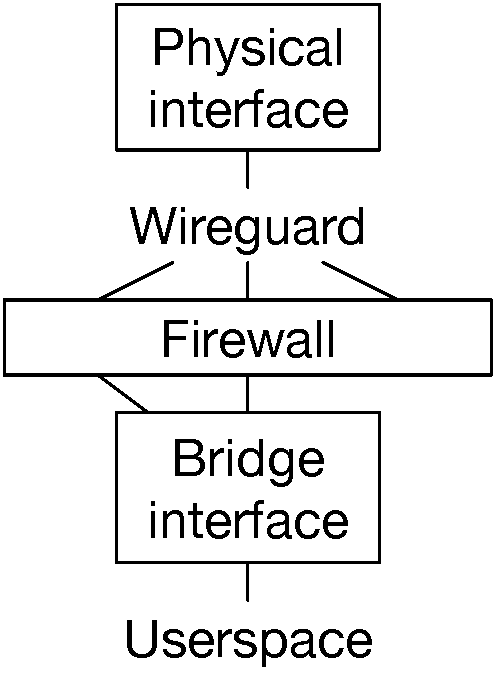
\includegraphics[width=0.28\textwidth]{metering-diagram.pdf}}
\end{wrapfigure}

Nodes create tunnels with each of their neighbors and can allow, block, or shape traffic on each tunnel, depending on payment. Wireguard creates a virtual interface for each tunnel. The virtual interfaces created by the tunnels of all the neighbors on one physical interface are bridged together into another virtual interface for Babel to run on. This preserves some per-interface optimizations made by Babel.

If payment over a neighbor’s payment channel stops, their packets are blocked by the firewall and are no longer forwarded.

Metering from the exit server to the home node is accomplished in the same way. There is also a Wireguard tunnel from the exit server to the home node for other reasons, namely privacy and and as part of Lightweight 4over6 \cite{4over6}. This tunnel provides a good control point for the exit server to cut service to the home node in the case of non-payment. 

\section{Network}
\label{sec:network}
The base primitive that Althea is built on is a pay-for-forward network. If all the mechanisms in the preceding sections work correctly, we have a network where nodes can pay each other very granularly for the service of forwarding data, and verify that the forwarding is happening correctly. This section deals with using such a network to provide the one of the most popular network services, internet access.

\begin{figure}[h]
\centering{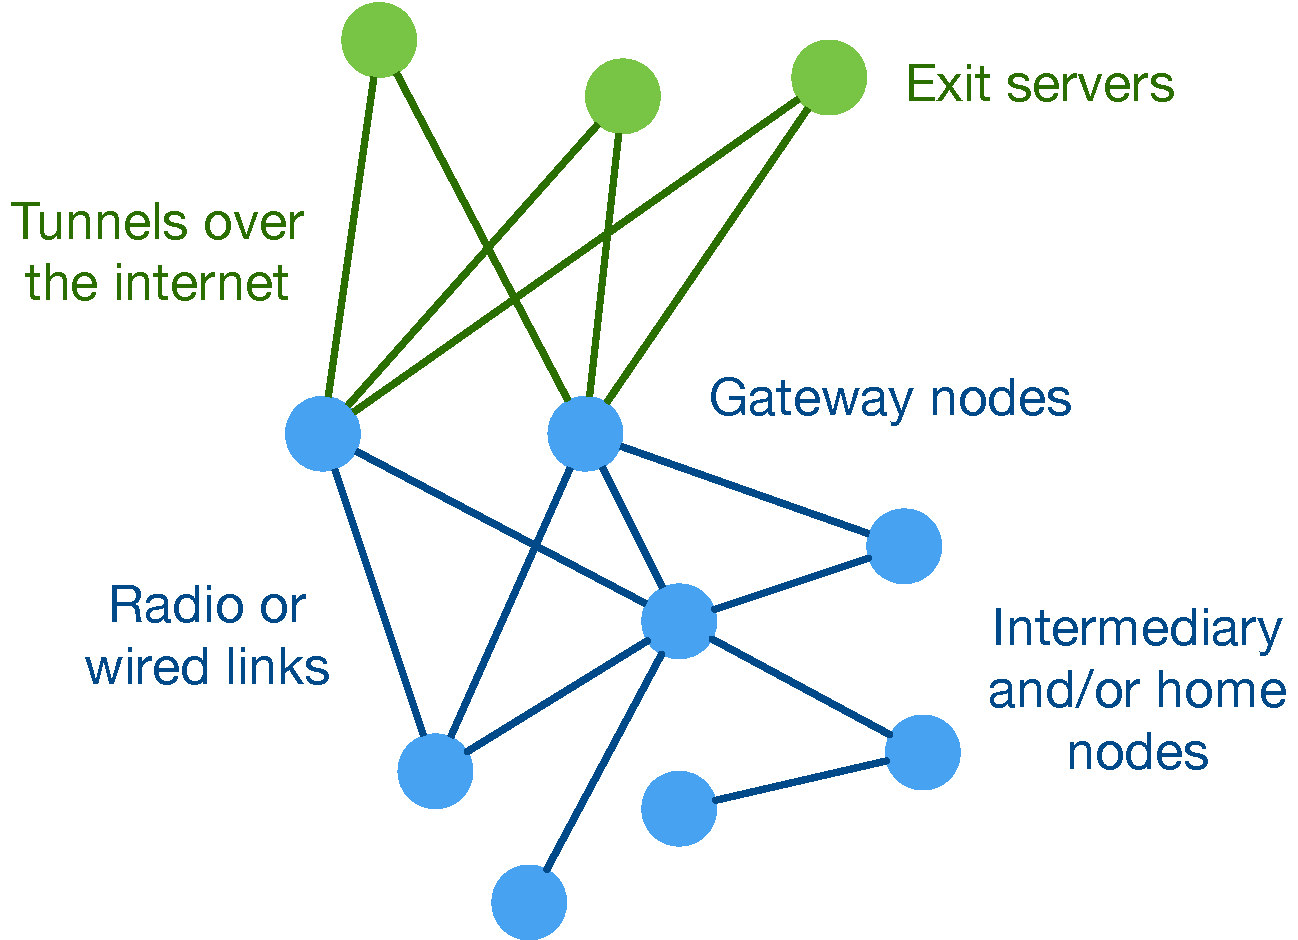
\includegraphics[width=0.58\textwidth]{node-types-diagram.pdf}}
\end{figure}

For a network to provide internet access, there must be at least one node that has a connection to the internet. Hopefully, there will be many. We call such a node a gateway node. A gateway node connects to an exit server over a tunnel. The tunnel creates a virtual interface which Babel is run on, treating it like any other link. The gateway node/exit server topology \cite{exittopology} is used by wlan slovenija \cite{wlanslovenija}, PeoplesOpen.net \cite{pplsopen}, and other community mesh networks.

Babel routes to destinations over tunnel connections just as well as it does over real connections. This means that the nodes do not have to do any kind of explicit gateway selection. Gateway nodes set a price and receive payment for routes to the exit server just like any other route. Home nodes are connected to chosen exit servers over encrypted tunnels, and receive internet access over these tunnels. The only thing that gateway and intermediary nodes see is encrypted traffic between home nodes and exit servers.

\subsection{Exit servers}
Exit servers perform almost all the functions of an ISP, except for actually carrying packets. This lets the other nodes in the network focus only on connectivity, while exit servers get paid for interfacing Althea to the rest of the internet, and to the business and legal worlds. Exit servers fuse Althea’s pseudonymous, trustless, cyptocurrency powered physical layer with our current internet and society. People who are good at providing connectivity can focus on providing connectivity, while exit servers deal with everything else. 

Exit servers:

\paragraph{Deal with public IP addresses}
Exit servers have public IP addresses and use them to route traffic for connected home nodes to and from the internet. They either perform NAT for home nodes or provision them with public IP addresses if the home nodes are performing NAT themselves (such as in schemes like Lightweight 4over6 \cite{4over6}). 

\paragraph{Provide encrypted tunnels}
All traffic between home nodes and exit servers is encapsulated in a tunnel and encrypted. This means that users of a Althea network only have to trust the exit server with their browsing history and unencrypted traffic. Neighbors who are routing traffic for them will only see encrypted packets going to an exit server.

\paragraph{Verify routes}
Our extensions to Babel allow nodes to verify routes between themselves and a destination. Exit servers are the destination for a home node’s outbound traffic, and the home nodes are destinations for the return traffic. Home nodes and exit servers work together to keep the nodes on the Althea network between them accurate. Home nodes are implicitly trusting exit servers to perform route verification accurately.

\paragraph{Deal with legal considerations}
We want it to be as easy as possible for someone to set up a gateway node. Part of this is relieving them of any legal worries related to the use of their connection. Any legal complaints related to the use of an Althea network can only be directed the exit servers, as they are the only ones routing traffic onto the internet and making it visible to the world. Gateway and intermediary nodes only ever see encrypted packets.

\paragraph{Pay for return traffic}
Home nodes pay their neighbors to forward traffic to the exit server they are using and onto the internet, but someone needs to pay for the traffic coming back. Home nodes give exit servers some money which the exit servers use to pay their neighbors for the return traffic. Payments from the home node to the exit server can be made in Althea tokens, which the exit server uses to pay its neighbors.

Alternately, payments to exit servers could be made with traditional payment systems such as credit cards. The exit server would then use this money to buy Althea tokens, which it would use to pay for incoming traffic sent to a particular home node. An exit server could also supply connected home nodes with the Althea tokens necessary to pay for their outgoing traffic. This could allow people to use Althea without having any understanding of cryptocurrency.

\begin{thebibliography}{99}

\bibitem{fcc}
\emph{Internet Access Services: Status as of June 30, 2016}\\
Industry Analysis and Technology Division Wireline Competition Bureau\\
\texttt{\url{http://transition.fcc.gov/Daily_Releases/Daily_Business/2017/db0503/DOC-344499A1.pdf}}\\
2017

\bibitem{wcn}
\emph{Wireless Community Networks:
An Alternative Approach for Nomadic Broadband Network Access}\\
Pantelis A. Frangoudis and George C. Polyzos, Athens University of Economics and Business Vasileios P. Kemerlis, Columbia University\\
\texttt{\url{https://www.cs.columbia.edu/~vpk/papers/wcn.commag11.pdf}}\\
2011

\bibitem{bellmanford}
\emph{Network Flow Theory}\\
Ford, L. R.\\
1956

\bibitem{etx}
\emph{A high-throughput path metric for multi-hop wireless networks}\\
De Couto, D., Aguayo, D., Bicket, J., and R. Morris\\
2003

\bibitem{bgp}
\emph{A Border Gateway Protocol 4 (BGP-4)}\\
Y. Rekhter, T. Li, S. Hares\\
\texttt{\url{https://tools.ietf.org/html/rfc4271}}\\
2006

\bibitem{babel}
\emph{The Babel Routing Protocol}\\
J. Chroboczek\\
\texttt{\url{https://tools.ietf.org/html/rfc6126}}\\
2011

\bibitem{btcwiki}
\emph{Micropayment Channel}\\
Bitcoin Wiki Contributors\\
\texttt{\url{https://bitcoin.org/en/developer-guide\#micropayment-channel}}\\
2014

\bibitem{bitcoinj}
\emph{[ANNOUNCE] Micro-payment channels implementation now in bitcoinj}\\
Mike Hearn\\
\texttt{\url{https://bitcointalk.org/index.php?topic=244656.0}}\\
2013

\bibitem{machinomy}
\emph{Machinomy}\\
\texttt{\url{https://machinomy.com}}\\
2017

\bibitem{ethermint}
\emph{Ethermint}\\
\texttt{\url{https://github.com/tendermint/ethermint}}\\
2016

\bibitem{ethereum}
\emph{A Next-Generation Smart Contract and Decentralized Application Platform}\\
Vitalik Buterin\\
\texttt{\url{https://github.com/ethereum/wiki/wiki/White-Paper}}\\
2014

\bibitem{erc20}
\emph{ERC: Token standard}\\
frozeman\\
\texttt{\url{https://github.com/ethereum/EIPs/issues/20}}\\
2015

\bibitem{80211i}
\emph{IEEE 802.11i-2004: Amendment 6: Medium Access Control (MAC) Security Enhancements}\\
2004

\bibitem{wireguard}
\emph{WireGuard: Next Generation Kernel Network Tunnel}\\
\texttt{\url{https://www.wireguard.io/papers/wireguard.pdf}}\\
2016

\bibitem{4over6}
\emph{Lightweight 4over6: An Extension to the Dual-Stack Lite Architecture}\\
Y. Cui, Q. Sun, M. Boucadair, T. Tsou, Y. Lee, I. Farrer\\
\texttt{\url{https://tools.ietf.org/html/rfc7596}}\\
2015

\bibitem{exittopology}
\emph{Mesh/Network topology}\\
\texttt{\url{https://sudoroom.org/wiki/Mesh/Network_topology}}\\
2015

\bibitem{wlanslovenija}
\emph{WLAN Slovenija}\\
\texttt{\url{https://wlan-si.net}}

\bibitem{pplsopen}
\emph{PeoplesOpen.net}\\
\texttt{\url{https://peoplesopen.net}}

\end{thebibliography}

\end{document}